% !TeX root = main.tex
\section{Summarizing Data Graphically}

\hypertarget{distribution-of-quantitative-data}{%
\subsection{Distribution of Quantitative
Data}\label{distribution-of-quantitative-data}}

\begin{itemize}
\item
  In data analysis, one goal is to describe \textbf{patterns} (known as
  the \textbf{distribution}) of the variable in the data set and create
  a useful summary about the set.
\item
  To describe patterns in data, we use descriptions of \textbf{shape},
  \textbf{center}, and \textbf{spread}. We also describe exceptions to
  the pattern. We call these exceptions \textbf{outliers}.
\end{itemize}

% \begin{figure}[h!]
  \begin{center}
    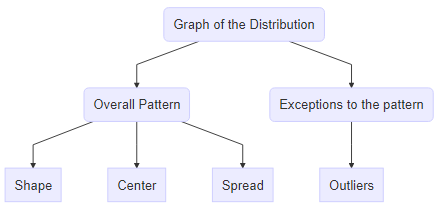
\includegraphics[width=\textwidth]{Figures/Graph-of-Distribution.png}
  \end{center}
% \end{figure}

\hypertarget{dot-plots}{%
\subsection{Dot Plots}\label{dot-plots}}

\begin{itemize}
\item
  A \textbf{dot plot} includes all values from the data set, with one
  dot for each occurrence of an observed value from the set.
\end{itemize}

\begin{example}
The data set contains 15 petal lengths of iris flower. Create a dot plot
to describe the distribution of petal lengths.

1.4, 1.4, 1.3, 1.5, 1.4, 1.7, 1.4, 1.5, 1.4, 1.5, 1.5, 1.6, 1.4, 1.1,
1.2
\end{example}
\vspace*{8\baselineskip}

\begin{exercise}
The data set contains the heights of 20 Black Cherry Trees. Create a dot
plot to describe the distribution of the heights.

64, 69, 71, 72, 74, 74, 75, 76, 76, 77, 78, 80, 80, 80, 80, 81, 82, 85,
86, 87
\end{exercise}
\vspace*{6\baselineskip}

\hypertarget{histograms}{%
\subsection{Histograms}\label{histograms}}

\begin{itemize}
\item
  A \textbf{histogram} divides values of a variable into
  \emph{equal-sized} intervals called \textbf{bins} (classes in some
  books) and uses a rectangular bar to show the \textbf{frequency
  (count)} of observations in each interval.
\item
  A \textbf{frequency distribution} is a table which contains bins,
  frequencies and/or \textbf{relative frequencies} which are proportions
  (percentage) defined by the formula \[
    \text{Relative frequency} =\frac{\text{Class frequency}}{\text{Sample size}}.
  \]
\item
  Each bin has a \textbf{lower bin limit}, which is the left endpoint of
  the interval, and an \textbf{upper bin limit}, which is the right
  endpoint of the interval.
\item
  The \textbf{bin width} is the distance between the lower (or upper)
  bin limits of two consecutive bins.
\item
  The difference between the maximum and the minimum data entries is
  called the \textbf{range}.
\item
  The \textbf{midpoint} of a bin is the half of the sum of the lower and
  upper limits of the bin.
\end{itemize}

\begin{example}
The following data set show the mpg (mile per gallon) of 30 cars.
Construct a frequency table and frequency histogram for the data set
using \(7\) bins.

21, 21, 22.8, 21.4, 18.7, 18.1, 14.3, 24.4, 22.8, 19.2, 17.8, 16.4,
17.3, 15.2, 10.4, 10.4, 14.7, 32.4, 30.4, 33.9, 21.5, 15.5, 15.2, 13.3,
19.2, 27.3, 26, 30.4, 15.8, 19.7
\end{example}
\vspace*{8\baselineskip}

\begin{remark}
\mbox{}
\begin{itemize}
\item
  Avoid histograms with large bin widths and small bin widths.
  \href{https://courses.lumenlearning.com/wmopen-concepts-statistics/chapter/histograms-2-of-4/}{See
  Histogram 2 of 4 in Concepts in Statistics for an interactive
  demonstration}
\item
  When bin width is no given, we may first determine the number of bins.
  If the number of bins is \(k\), then we choose a number with the same
  or one more decimal place that is greater than
  \(\frac{\text{range}}{k}\), but no more than
  \(\frac{\text{range}}{k-1}\) as the bin width. This is to avoid that
  the last bin limit is too much bigger than the max.

  To determine the number of bins, there are some ``rules of thumb''.
  For example, the Rice rule takes the bin number
  \(k = \lceil 2n^{1/3}\rceil\), where \(\lceil 2n^{1/3}\rceil\) is the
  roundup of \(2n^{1/3}\).

  See the
  \href{https://www.statisticshowto.datasciencecentral.com/choose-bin-sizes-statistics/}{Statistic
  How To} page for more discussion on choosing bin width.
\item
  The convenient starting point should not be too much smaller than the
  min. The starting points together with the bin width affects the shape
  of the histogram. It'd be better to experiment with different choices
  of the starting point and the bin width.
\item
  The area of a bar represents the relative frequency for the bin. There
  should be \emph{no space} between any two bars.
\end{itemize}

\end{remark}

\begin{exercise}
The following data set show the petal length of 20 irises. Construct a
frequency table and frequency histogram for the data set using 6 bins.

1.4, 5.4, 1.2, 4.5, 6.1, 1.5, 4.7, 1.4, 5.6, 5.2, 1.3, 6.3, 5.1, 5.6, 5,
6.7, 1.4, 1.6, 1.5, 1.5
\end{exercise}
\vspace*{8\baselineskip}

\hypertarget{common-descriptions-of-shape-distribution}{%
\subsection{Common Descriptions of Shape
Distribution}\label{common-descriptions-of-shape-distribution}}

\begin{itemize}
\item
  \textbf{Right skewed} (or reverse \(J\)-shaped): A right-skewed
  distribution has a lot of data at lower variable values. (Example: the
  histogram example.)
\item
  \textbf{Left skewed} (or \(J\)-shaped): A left skewed distribution has
  a lot of data at higher variable values with smaller amounts of data
  at lower variable values.
\item
  \textbf{Symmetric with a central peak (or bell-shaped)}: A central
  peak with a tail in both directions. A bell-shaped distribution has a
  lot of data in the center with smaller amounts of data tapering off in
  each direction. (Example: the petal length example.)
\item
  \textbf{Uniform}: A rectangular shape, the same amount of data for
  each variable value.
\end{itemize}

\begin{exercise}
Statistics are used to compare and sometimes identify authors. The
following lists shows a simple random sample that compares the letter
counts for three authors.

Terry: 7, 9, 3, 3, 3, 4, 1, 3, 2, 2

Davis: 3, 4, 4, 4, 1, 4, 5, 2, 3, 1

Maris: 2, 3, 4, 4, 4, 6, 6, 6, 8, 3

Create a dot plot for each sample and describe the shape of the
distribution of each sample.
\end{exercise}
\vspace*{5\baselineskip}

\hypertarget{measure-of-centers}{%
\subsection{Measure of Centers}\label{measure-of-centers}}

\begin{itemize}
\item
  \textbf{Mean}: The mean is the average, this is the quotient of the
  total sum by the total number.
\item
  \textbf{Median}: The median is a value that separate the data into the
  lower half and the upper half. To calculate the median, sort the data
  first. If the number of data values is odd, the median is the middle
  value. Otherwise, the median is the mean of the middle two values.
\item
  \textbf{Mode}: The mode is the value that has the most occurrence in
  the data set.
\item
  Use the \emph{mean} as a measure of center only for distributions that
  are \emph{reasonably symmetric} with a central peak. When outliers are
  present, the mean is not a good choice.
\item
  Use the \emph{median} as a measure of center for all \emph{other
  cases}.
\item
  We need to use a graph to determine the shape of the distribution. So
  graph the data first.
\end{itemize}
\vspace*{-\baselineskip}

\begin{exercise}
A student survey was conducted at a major university. The following
histogram shows distribution of alcoholic beverages consumed in a
typical week. 

1. What is the typical number of drinks a student has
during a week? 

2. Do the data suggest that drinking is a problem in this
university?

\begin{fullwidth}
\begin{center}
  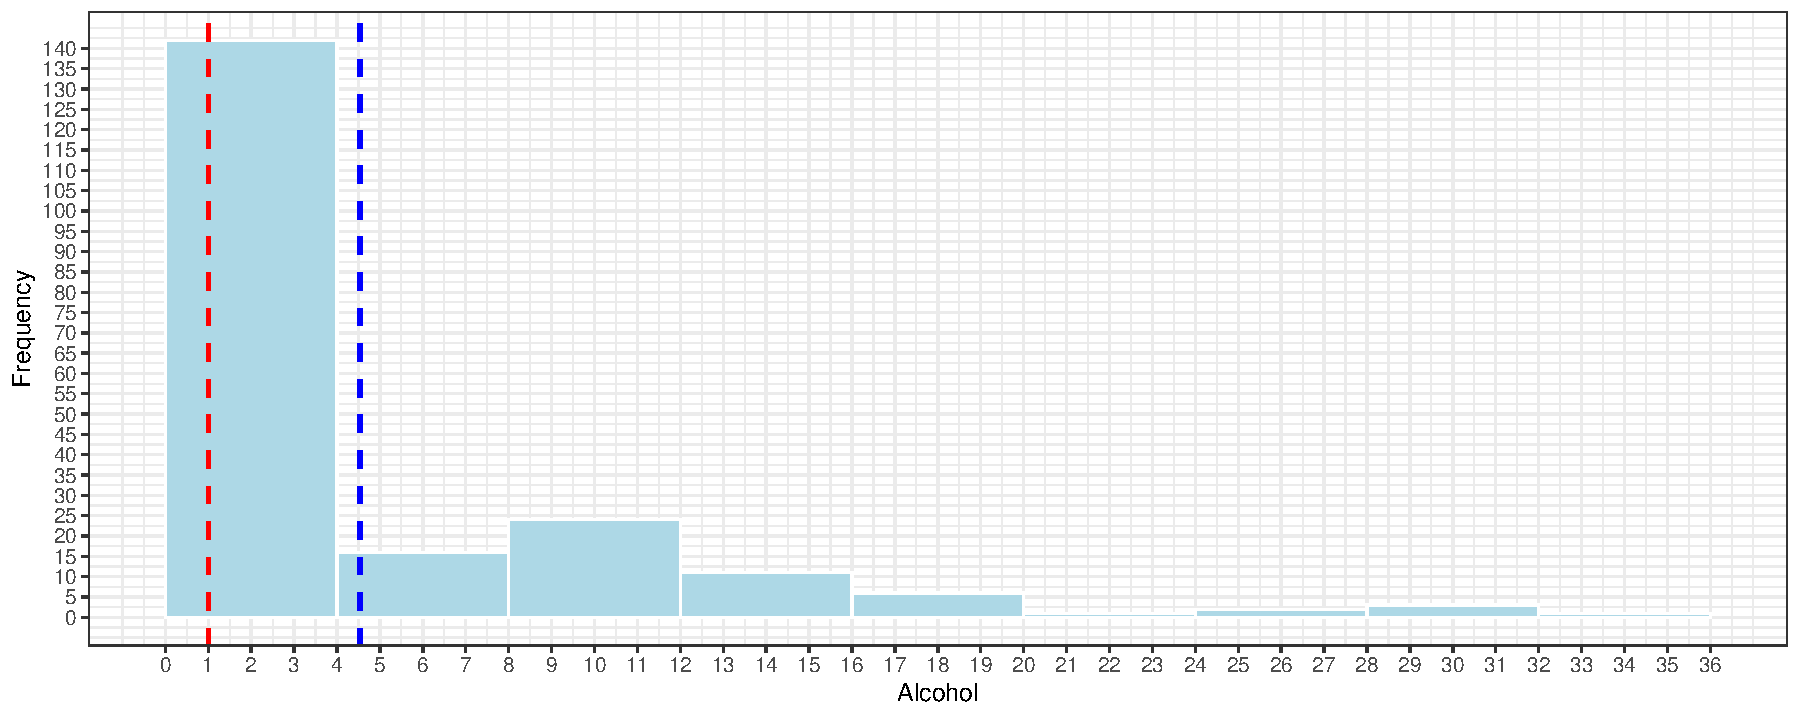
\includegraphics[width=\linewidth]{figure-latex/unnamed-chunk-2-6-1}
\end{center}
\end{fullwidth}
\end{exercise}
\vspace*{5\baselineskip}

\hypertarget{pie-charts}{%
\subsection{Pie Charts}\label{pie-charts}}

\begin{itemize}
\item
  A \textbf{pie chart} is a pie with sectors represents categories and
  the area of each sector is proportional to the frequency of each
  category.

  \begin{itemize}
  \item
    The \textbf{frequency} of a category is the number of occurrences of
    elements in the category.
  \item
    The proportion of a frequency to the size of the population or the
    sample is also called the \textbf{relative frequency}.
  \end{itemize}
\end{itemize}

\begin{example}
The counts of majors of 100 students in a sample are shown in the table.
Use a pie chart to organize the data.

\begin{table}[h!]
  \begin{small}
      \begin{tabular}[c]{l|l}
        \hline
        \multicolumn{1}{c}{\textbf{Grade}} & 
        \multicolumn{1}{c}{\textbf{Frequency (Counts)}} \\
        \hline
        Art & 30 \\
        Engineering & 50 \\
        Science & 20 \\
        \hline
      \end{tabular}
  \end{small}
\end{table}
\end{example}
\vspace*{5\baselineskip}

\begin{exercise}
The following data table summarize passengers on Titanic. Using a pie
chart to describe the data table.

\begin{table}[h!]
  \begin{small}
      \begin{tabular}[c]{l|l}
        \hline
        \multicolumn{1}{c}{\textbf{Class}} & 
        \multicolumn{1}{c}{\textbf{Passengers}} \\
        \hline
        1st & 325 \\
        2nd & 285 \\
        3rd & 706 \\
        Crew & 885 \\
        \hline
      \end{tabular}
  \end{small}
\end{table}

\end{exercise}
\vspace*{5\baselineskip}


\hypertarget{lab-2-summarizing-data-graphically}{%
\subsection{Lab 2: Summarizing Data
Graphically}\label{lab-2-summarizing-data-graphically}}

\hypertarget{create-frequency-tables}{%
\subsubsection{Create Frequency Tables}\label{create-frequency-tables}}

In Excel, to create a frequency table for a data array, we need a bin
array which is used to split the date set into smaller intervals. The
values in a bin array in Excel are (upper) boundaries of intervals. With
a data array and a bin array, we can use the Excel function
\textsf{FREQUENCY\ (data\_array,\ bins\_array)} to create a frequency
table.

Suppose the data set is in column A and the bin array is in column B.
Here is how to create a frequency table using the function
\textsf{FREQUENCY\ (data\_array,\ bins\_array)}:

\begin{enumerate}[sepno]
\item
  In column C, right to the smallest value of the bin array enter
  \textsf{=FREQUENCY(}
\item
  select the data values
\item
  in the formula bar, enter the symbol comma \textsf{,}
\item
  select the bin array
\item
  in the formula bar, enter \textsf{)}.
\end{enumerate}

Hit the \textsf{Enter}, you will get a frequency table.

\begin{remark}

\begin{enumerate}[sepno]
\item
  In this formula, the values in a bin array should be first \(k-1\)
  upper class limits (or the last \(k-1\) lower class limits), where
  \(k\) is the number of bins. In Excel, if the bin array consists of
  30, 40, and 50, then the bins will be \((-\infty,30]\), \((30,40]\),
  \((40, 50]\), \((50, \infty)\).
\item
  In older version of Excel, you may have to highlight cells for
  frequencies first, enter the \textsf{FREQUENCY} function secondly, and
  then hit \textsf{Ctrl+Shift+Enter} (or \textsf{Cmd+Shift+Enter} on
  Mac).
\end{enumerate}

\end{remark}

\begin{exercise}
  Create a frequency table for the following data using the bin width 10.

  31, 32, 32, 33, 35, 36, 37, 37, 38, 38, 39, 40, 40, 40, 42, 42, 43, 43, 45, 45, 46, 47, 48, 48, 51, 55, 55, 56, 60, 60, 61, 66
\end{exercise}
\vspace*{6\baselineskip}

\hypertarget{creating-charts-in-excel}{%
\subsubsection{Creating Charts in Excel}\label{creating-charts-in-excel}}

Excel has many built-in chart functions. To create a charts,

\begin{enumerate}[sepno]
\item
  Select the data array/table
\item
  Under the \textsf{Insert} tab, click on an appropriate chart in the
  \textsf{Charts} command set.
\end{enumerate}

The appearance of chart can be changed after being created.

\begin{exercise}
  The counts of majors of 50 students in a sample are shown in the table.
Use a pie chart to organize the data.

\begin{tabular}[c]{l|l}
  \hline
  \multicolumn{1}{c}{\textbf{Grade}} & 
  \multicolumn{1}{c}{\textbf{Count}} \\
  \hline
  Art & 10 \\
  Engineering & 25 \\
  Mathematics & 15 \\
  \hline
\end{tabular}

\end{exercise}

\vspace*{6\baselineskip}

\hypertarget{create-histogram-charts-in-excel}{%
\subsubsection{Create a Histogram in
Excel}\label{create-histogram-charts-in-excel}}

\begin{enumerate}[sepno]
\item
  Select the data
\item
  On the \textsf{Insert} tab, in the \textsf{Charts} group, from the
  \textsf{Insert\ Statistic\ Chart} dropdown list, select
  \textsf{Histogram}:

  \textbf{Note:} The histogram contains a special first bin which always
  contains the smallest number. This is different from many textbooks.
\end{enumerate}

To \textbf{format the histogram chart} is similar to format a Pie chart.
For example, you can change bin width from \textsf{Format\ Axis}.

\begin{enumerate}[sepno]
\item
  Right-click on the horizontal axis and choose \textsf{Format\ Axis} in
  the popup menu:
\item
  In the \textsf{Format\ Axis} pane, on the \textsf{Axis\ Options} tab,
  you may try different options for bins.
\end{enumerate}

\begin{remark}

\begin{itemize}
\item
  Excel using a different convention to create histogram. The first bin
  is a closed interval and other bins are left open and right closed
  intervals.
\item
  Select the \textbf{Overflow bin} checkbox and type the number, all
  values above this number will be added to the last bin.
\item
  Select the \textbf{Underflow bin} checkbox and type the number, all
  values below and equal to this number will be added to the first bin.
\item
  Histograms show the shape and the spread of quantitative data. For
  categorical data, discrete by its definition, bar charts are usually
  used to represent category frequencies.
\end{itemize}

\end{remark}

\hypertarget{create-histogram-charts-in-excel-using-the-analysis-toolpak}{%
\subsubsection{\texorpdfstring{Create Histogram Charts in Excel using the
\textsf{Analysis\ ToolPak}}{Create Histogram Charts in Excel using the Analysis ToolPak}}\label{create-histogram-charts-in-excel-using-the-analysis-toolpak}}

Suppose your data set is in \textsf{Column\ A} in Excel.

\begin{itemize}
\item
  In the cell \textsf{B1}, put the \emph{first lower bin limit}, which
  is a number slightly less than the minimum but has more decimal places
  than the data set.
\item
  Create upper bin limits in column C.
\item
  In Data menu, look for the Data Analysis ToolPak (if not, go to File
  $\rightarrow$ Options $\rightarrow$ Add-ins $\rightarrow$ Manage
  Excel Add-ins, check Analysis ToolPak). In the popup windows, find
  Histogram.
\item
  In the input range, select your data set. In the bin range, select
  upper bins.
\item
  Check Chart Output and hit OK. You will see the frequency table and
  histogram in Sheet 2.
\item
  Change the gap between bars. Right click a bar and choose
  \textsf{Format\ Data\ Series...} and change the \textsf{Gap\ Width} to
  2\% or 1\%.
\end{itemize}

\hypertarget{how-to-create-a-dotplot-in-excel}{%
\subsubsection{How to Create a Dotplot in
Excel}\label{how-to-create-a-dotplot-in-excel}}

\begin{itemize}
\item
  If you have a raw data set, follow the same procedure a creating a
  histogram but with a bin width equal the same accuracy of the data.
  For example, if you data set consists of integers, then choose 1 as
  the bin-width.
\item
  Change the format of bars in the histogram.

  \begin{itemize}
  \item
    Right click a bar and select \textsf{Format\ Data\ Series...}.
  \item
    Find \textsf{Fill\ \&\ Line} and select both
    \textsf{Picture\ or\ texture\ fill} and
    \textsf{Stack\ and\ Scale\ with}.
  \item
    Click the button \textsf{Online...} and input \emph{dot} in
    \textsf{search\ bing} and hit enter.
  \item
    Select a picture you like and you will get a dot-plot. 
  \end{itemize}
\end{itemize}

\begin{exercise}
Use Excel to complete the following tasks:
\begin{enumerate}[sepno]
\item
  Create a random sample of 30 two-digit integers.
\item
  Create a histogram with 6 bins for the sample.
\item
  Describe the shape of the distribution of the sample of 30 two-digit
  integers.
\end{enumerate}
\end{exercise}